\documentclass{article}

% if you need to pass options to natbib, use, e.g.:
% \PassOptionsToPackage{numbers, compress}{natbib}
% before loading nips_2016
%
% to avoid loading the natbib package, add option nonatbib:
% \usepackage[nonatbib]{nips_2016}


\usepackage{dsfont}

% to compile a camera-ready version, add the [final] option, e.g.:
\usepackage{nips_2017}

\usepackage[utf8]{inputenc} % allow utf-8 input
\usepackage[T1]{fontenc}    % use 8-bit T1 fonts
\usepackage{hyperref}       % hyperlinks
\usepackage{url}            % simple URL typesetting
\usepackage{booktabs}       % professional-quality tables
\usepackage{amsfonts}       % blackboard math symbols
\usepackage{nicefrac}       % compact symbols for 1/2, etc.
\usepackage{microtype}      % microtypography

\usepackage{listings}
\usepackage{amsthm}
% use Times
\usepackage{times}
% For figures
\usepackage{graphicx} % more modern
%\usepackage{epsfig} % less modern
\usepackage{subfig} 
\usepackage{fancyvrb}


\usepackage{caption}
\usepackage{subcaption}

\fvset{fontsize=\footnotesize}

\usepackage{amssymb}
\usepackage{listings}
\usepackage{wrapfig}
\usepackage{tabularx}


\usepackage{verbatim}
 \usepackage{booktabs}
 % For algorithms
\usepackage{algorithm}
\usepackage{algorithmic}
\usepackage{tikz}
% As of 2011, we use the hyperref package to produce hyperlinks in the
% resulting PDF.  If this breaks your system, please commend out the
% following usepackage line and replace \usepackage{icml2016} with
% \usepackage[nohyperref]{icml2016} above.
\usepackage{amsmath}
\usepackage{hyperref}
\DeclareMathOperator*{\argmin}{arg\,min} % thin space, limits underneath in displays
\DeclareMathOperator{\argmin}{argmin} % no space, limits underneath in displays



% Packages hyperref and algorithmic misbehave sometimes.  We can fix
% this with the following command.

\newcommand{\Expect}{\mathds{E}} %{{\rm I\kern-.3em E}}
\newcommand{\probability}{\mathds{P}} %{{\rm I\kern-.3em P}}

\newtheorem{proposition}{Proposition}

\newcommand\modt{\stackrel{\mathclap{\normalfont 2}}{\equiv}}


\title{Supplement to: Inferring Graphics Programs from Images}

% The \author macro works with any number of authors. There are two
% commands used to separate the names and addresses of multiple
% authors: \And and \AND.
%
% Using \And between authors leaves it to LaTeX to determine where to
% break the lines. Using \AND forces a line break at that point. So,
% if LaTeX puts 3 of 4 authors names on the first line, and the last
% on the second line, try using \AND instead of \And before the third
% author name.

\author{
Kevin Ellis \\
Brain and Cognitive Sciences\\
MIT\\
%Pittsburgh, PA 15213 \\
\texttt{ellisk@mit.edu} \\
Daniel Ritchie\\
Department of Computer Science\\
Brown
\And
Armando Solar-Lezama \\
  CSAIL\\
MIT \\
\texttt{asolar@csail.mit.edu} \\
\And
Joshua B. Tenenbaum \\
Brain and Cognitive Sciences\\
MIT\\
\texttt{jbt@mit.edu} \\
}

\begin{document}
% \nipsfinalcopy is no longer used

\maketitle

\section{Neural network architecture}

\subsection{Convolutional network}
The convolutional network takes as input 2 $256\times 256$ images
represented as a $2\times 256\times 256\times$ volume. These are
passed through two layers of convolutions separated by ReLU
nonlinearities and max pooling:
\begin{itemize}
\item Layer 1: 20 $8\times 8$ convolutions, 2 $16\times 4$ convolutions, 2 $4\times 16$ convolutions. Followed by $8\times 8$ pooling with a stride size of 4.
\item Layer 2: 10 $8\times 8$ convolutions. Followed by $4\times 4$ pooling with a stride size of 4.
\end{itemize}
Training takes a little bit less than a day on a Nvidia TitanX GPU.
The network was trained on $10^5$ synthetic examples.

\subsection{Autoregressive decoding of drawing commands}

Given the image features $f$, we predict the first token using logistic regression:
\begin{equation}
  \probability [T_1]\propto W_{T_1}f
\end{equation}
where $W_{T_1}$ is a learned weight matrix.

Subsequent tokens are predicted as:
\begin{equation}
  \probability [T_n|T_{1:(n - 1)}]\propto \text{MLP}_{T_1,n}(I \otimes \bigotimes_{j < n} \text{oneHot}(T_j))
\end{equation}
Thus each token of each drawing primitive has its own learned MLP.
For predicting the coordinates of lines we found that using 32 hidden nodes with sigmoid activations worked well;
for other tokens the MLP's are just logistic regression (no hidden nodes).

\subsection{A learned likelihood surrogate}

Our architecture for
$L_{\text{learned}}(\text{render}(T_1)|\text{render}(T_2))$ has the
same series of convolutions as the network that predicts the next
drawing command. We train it to predict two scalars: $|T_1 - T_2|$ and
$|T_2 - T_1|$.  These predictions are made using linear regression
from the image features followed by a ReLU nonlinearity; this
nonlinearity makes sense because the predictions can never be negative
but could be arbitrarily large positive numbers.

We train this network by sampling random synthetic scenes for $T_1$,
and then perturbing them in small ways to produce $T_2$.
We minimize the squared loss between the network's prediction and the ground truth symmetric differences.
$T_1$ is rendered in a ``simulated hand drawing'' style which we describe next.

\section{Simulating hand drawings}

We introduce noise into the \LaTeX~rendering process by:

\begin{itemize}
\item Rescaling the image intensity by a factor chosen uniformly at random from $[0.5,1.5]$
\item Translating the image by $\pm 3$ pixels chosen uniformly random
\item Rendering the \LaTeX~using the \verb|pencildraw| style,
  which adds random perturbations to the paths drawn by \LaTeX in a way designed to resemble a pencil.
\item Randomly perturbing the positions and sizes of primitive  \LaTeX drawing commands
  \end{itemize}

\section{Generating synthetic training data}

I need to describe the procedure that I used to sample the scenes. it's pretty involved

\section{The cost function for programs}

We seek the minimum cost program which evaluates to (produces the drawing primitives in) an execution trace $T$:
\begin{equation}
  \text{program}(T) = \argmin_{\substack{p\in \text{DSL}\\p \text{ evaluates to } T}} \text{cost}(p)\label{programObjective}
\end{equation}

Programs incur a cost of 1 for each command (primitive drawing action,
loop, or reflection).  They incur a cost of $\frac{1}{3}$ for each
unique coefficient they use in a linear transformation beyond the
first coefficient. This encourages reuse of coefficients, which leads
to code that has translational symmetry; rather than provide a
translational symmetry operator as we did with reflection, we modify
what is effectively a prior over the space of program so that it tends
to produce programs that have this symmetry.

Programs also incur a cost of 1 for having loops of constant length 2;
otherwise there is often no pressure from the cost function to explain
a repetition of length to as being a reflection rather a loop.

%% \section{Neural networks for guiding SMC}



%% Let $L(\cdot | \cdot):\text{image}^2\to \mathcal{R}$ be our likelihood
%% function: it takes two images, an observed target image and a
%% hypothesized program output, and gives the likelihood of the observed
%% image conditioned on the program output. We want to sample from:
%% \begin{equation}
%% \probability [p|x]  \propto L(x | \text{render}(p)) \probability [p]
%% \end{equation}
%% where $\probability [p]$ is the prior probability of program $p$, and $x$ is the observed image.

%% Let $p$ be a program with $L$ lines, which we will write as $p = (p_1,p_2,\cdots,p_L)$. Assume the prior factors into:
%% \begin{equation}
%%   \probability [p]\propto \prod_{l\leq L}\probability [p_l]
%% \end{equation}
%% Define the distribution $q_L(\cdot)$, which happens to be proportional to the above posterior:
%% \begin{equation}
%%   q_L(p_1,p_2,\cdots,p_{L - 1},p_L)\propto q_{L - 1}(p_1,p_2,\cdots,p_{L - 1})\times \frac{L(x | \text{render}(p_1,p_2,\cdots,p_{L - 1},p_L))}{L(x | \text{render}(p_1,p_2,\cdots,p_{L - 1}))}\times\probability [p_L]
%% \end{equation}
%% Now suppose we have some samples from $q_{L - 1}(\cdot)$, and that we
%% then sample a $p_L$ from a distribution proportional to $\frac{L(x |
%%   \text{render}(p_1,p_2,\cdots,p_{L - 1},p_L))}{L(x |
%%   \text{render}(p_1,p_2,\cdots,p_{L - 1}))}\times\probability [p_L]$.
%% The resulting programs $p$ are distributed according to $q_L$, and so
%% are also distributed according to $\probability [p|x]$.

%% How do we sample $p_L$ from a distribution proportional to $\frac{L(x
%%   | \text{render}(p_1,p_2,\cdots,p_{L - 1},p_L))}{L(x |
%%   \text{render}(p_1,p_2,\cdots,p_{L - 1}))}\times\probability [p_L]$?
%% We have a neural network that takes as input the target image $x$ and
%% the program so far, and produces a distribution over next lines of
%% code ($p_L$).  We write $\text{NN}(p_L | p_1,\cdots,p_{L - 1};x)$ for
%% the distribution output by the neural network. So we can sample from NN and then weight the samples by:
%% \begin{equation}
%%   w(p_L) = \frac{\probability [p_L]}{\text{NN}(p_L | p_1,\cdots,p_{L - 1};x)}\times \frac{L(x | \text{render}(p_1,p_2,\cdots,p_{L - 1},p_L))}{L(x | \text{render}(p_1,p_2,\cdots,p_{L - 1}))}
%% \end{equation}
%% Then we can resample from these now weighted samples to get a new
%% population of particles (here programs are particles), where each
%% program now has $L$ lines instead of $L - 1$.

%% This procedure can be seen as a particle filter, where each successive
%% latent variable is another line of code, and the emission
%% probabilities are successive ratios of likelihoods under $L(\cdot |
%% \cdot)$.


%%   \begin{algorithm}[tb]
%%    \caption{Neurally guided SMC}
%%    \label{guideAlgorithm}
%% \begin{algorithmic}
%%   \STATE {\bfseries Input:} Neural network NN, beam size $N$, maximum length $L$, target image $x$
%%   \STATE {\bfseries Output:} Samples of the program trace
%%   \STATE Set $B_0 = \{\text{empty program}\}$
%%   \FOR{$1\leq l\leq L$}
%%   \FOR{$1\leq n\leq N$}
%%   \STATE{ $p_n\sim \text{Uniform}(B_{l - 1})$}
%%   \STATE{ $p'_{n}\sim \text{NN}(\text{render}(p),x)$}
%%   \STATE{ Define $r_n = p'_n\cdot p_n$}
%%   \STATE{ Set $\tilde{w}(r_n) = \frac{L(x|r_n)}{L(x|p_n)}\times\frac{\probability [p'_n]}{\probability [p'_n = \text{NN}(\text{render}(p),x)]}$}
%%   \ENDFOR
%%   \STATE{ Define $w(p) = \frac{\tilde{w}(p)}{\sum_{p'}\tilde{w}(p')}$}
%%   \STATE{ Set $B_l$ to be $N$ samples from $r_n$ distributed according to $w(\cdot)$}
%%   \ENDFOR
%%   \STATE {\bfseries return} $\{p : p\in B_{l\leq L}, p \text{ is finished}\}$
%% \end{algorithmic}
%%   \end{algorithm}

\section{Full results on drawings data set}

Below we show our full data set of drawings. The leftmost column is a hand drawing. The middle column is a rendering of the most likely trace discovered by the neurally guided SMC sampling scheme. The rightmost column is the program we synthesized from a ground truth execution trace of the drawing.

            \begin{tabular}{lll}
    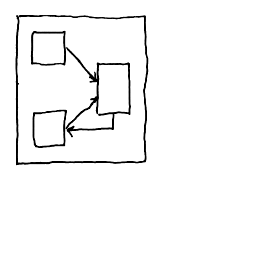
\includegraphics[width = 5cm]{../TikZ/drawings/expert-0.png}&
            \includegraphics[width = 5cm]{../TikZ/drawings/expert-0-parses/0.png}&
    
        \begin{minipage}{10cm}
        \begin{verbatim}
line(6,2,6,3,
arrow = False,solid = True);
line(6,2,3,2,
arrow = True,solid = True);
reflect(reflect(y = 9)){
line(3,2,5,4,
arrow = True,solid = True);
rectangle(0,0,8,9);
rectangle(5,3,7,6);
rectangle(1,1,3,3)
}
        \end{verbatim}
\end{minipage}

    \end{tabular}        
            \\

            \begin{tabular}{lll}
    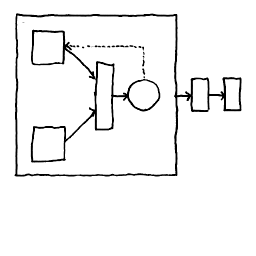
\includegraphics[width = 5cm]{../TikZ/drawings/expert-1.png}&
            \includegraphics[width = 5cm]{../TikZ/drawings/expert-1-parses/0.png}&
    
        \begin{minipage}{10cm}
        \begin{verbatim}
Solver timeout
        \end{verbatim}
\end{minipage}

    \end{tabular}        
            \\

            \begin{tabular}{lll}
    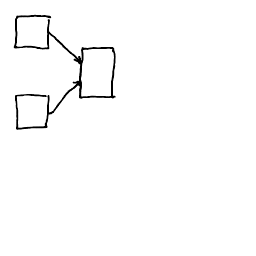
\includegraphics[width = 5cm]{../TikZ/drawings/expert-2.png}&
            \includegraphics[width = 5cm]{../TikZ/drawings/expert-2-parses/0.png}&
    
        \begin{minipage}{10cm}
        \begin{verbatim}
rectangle(4,2,6,5);
reflect(reflect(y = 7)){
line(2,6,4,4,
arrow = True,solid = True);
rectangle(0,0,2,2)
}
        \end{verbatim}
\end{minipage}

    \end{tabular}        
            \\

            \begin{tabular}{lll}
    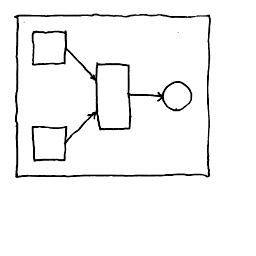
\includegraphics[width = 5cm]{../TikZ/drawings/expert-3.png}&
            \includegraphics[width = 5cm]{../TikZ/drawings/expert-3-parses/0.png}&
    
        \begin{minipage}{10cm}
        \begin{verbatim}
circle(10,5);
line(7,5,9,5,
arrow = True,solid = True);
rectangle(5,3,7,7);
rectangle(0,0,12,10);
reflect(reflect(y = 10)){
line(3,8,5,6,
arrow = True,solid = True);
rectangle(1,7,3,9)
}
        \end{verbatim}
\end{minipage}

    \end{tabular}        
            \\

            \begin{tabular}{lll}
    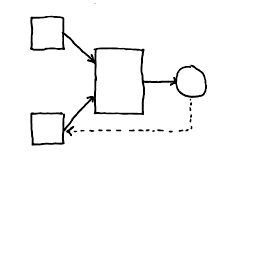
\includegraphics[width = 5cm]{../TikZ/drawings/expert-4.png}&
            \includegraphics[width = 5cm]{../TikZ/drawings/expert-4-parses/0.png}&
    
        \begin{minipage}{10cm}
        \begin{verbatim}
circle(10,4);
line(10,1,2,1,
arrow = True,solid = False);
line(10,1,10,3,
arrow = False,solid = False);
line(7,4,9,4,
arrow = True,solid = True);
reflect(reflect(y = 8)){
line(2,7,4,5,
arrow = True,solid = True);
rectangle(4,2,7,6);
rectangle(0,6,2,8)
}
        \end{verbatim}
\end{minipage}

    \end{tabular}        
            \\

            \begin{tabular}{lll}
    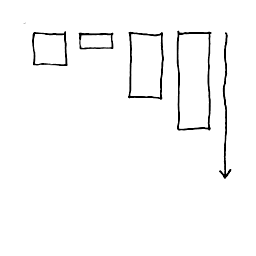
\includegraphics[width = 5cm]{../TikZ/drawings/expert-5.png}&
            \includegraphics[width = 5cm]{../TikZ/drawings/expert-5-parses/0.png}&
    
        \begin{minipage}{10cm}
        \begin{verbatim}
Solver timeout
        \end{verbatim}
\end{minipage}

    \end{tabular}        
            \\

            \begin{tabular}{lll}
    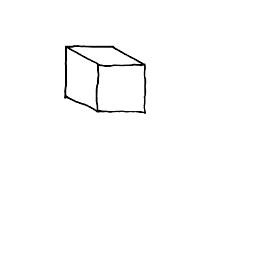
\includegraphics[width = 5cm]{../TikZ/drawings/expert-6.png}&
            \includegraphics[width = 5cm]{../TikZ/drawings/expert-6-parses/0.png}&
    
        \begin{minipage}{10cm}
        \begin{verbatim}
line(0,1,2,0,
arrow = False,solid = True);
for (i < 3){
if (i > 0){
line(3*i + -3,4,3*i + -1,3,
arrow = False,solid = True);
line(0,3*i + -2,3*i + -3,4,
arrow = False,solid = True)
}
rectangle(2,0,5,3)
}
        \end{verbatim}
\end{minipage}

    \end{tabular}        
            \\

            \begin{tabular}{lll}
    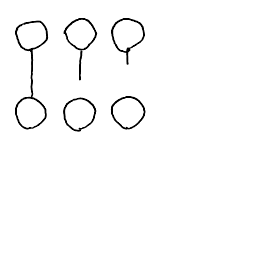
\includegraphics[width = 5cm]{../TikZ/drawings/expert-7.png}&
            \includegraphics[width = 5cm]{../TikZ/drawings/expert-7-parses/0.png}&
    
        \begin{minipage}{10cm}
        \begin{verbatim}
for (i < 3){
circle(-3*i + 7,1);
circle(-3*i + 7,6);
line(-3*i + 7,-1*i + 4,-3*i + 7,5,
arrow = False,solid = True)
}
        \end{verbatim}
\end{minipage}

    \end{tabular}        
            \\

            \begin{tabular}{lll}
    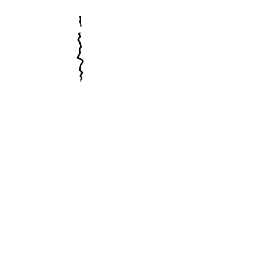
\includegraphics[width = 5cm]{../TikZ/drawings/expert-8.png}&
            \includegraphics[width = 5cm]{../TikZ/drawings/expert-8-parses/0.png}&
    
        \begin{minipage}{10cm}
        \begin{verbatim}
line(0,0,0,4,
arrow = False,solid = True)
        \end{verbatim}
\end{minipage}

    \end{tabular}        
            \\

            \begin{tabular}{lll}
    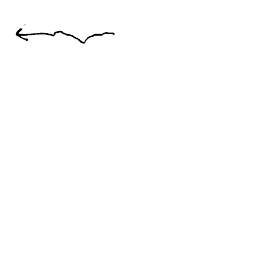
\includegraphics[width = 5cm]{../TikZ/drawings/expert-9.png}&
            \includegraphics[width = 5cm]{../TikZ/drawings/expert-9-parses/0.png}&
    
        \begin{minipage}{10cm}
        \begin{verbatim}
line(6,0,0,0,
arrow = True,solid = True)
        \end{verbatim}
\end{minipage}

    \end{tabular}        
            \\

            \begin{tabular}{lll}
    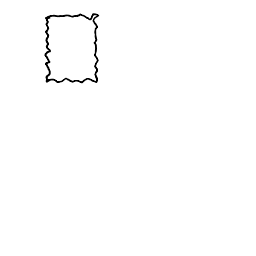
\includegraphics[width = 5cm]{../TikZ/drawings/expert-10.png}&
            \includegraphics[width = 5cm]{../TikZ/drawings/expert-10-parses/0.png}&
    
        \begin{minipage}{10cm}
        \begin{verbatim}
rectangle(0,0,3,4)
        \end{verbatim}
\end{minipage}

    \end{tabular}        
            \\

            \begin{tabular}{lll}
    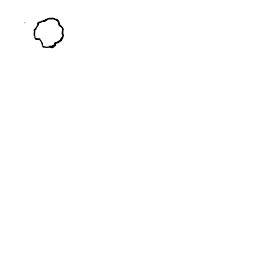
\includegraphics[width = 5cm]{../TikZ/drawings/expert-11.png}&
            \includegraphics[width = 5cm]{../TikZ/drawings/expert-11-parses/0.png}&
    
        \begin{minipage}{10cm}
        \begin{verbatim}
circle(1,1)
        \end{verbatim}
\end{minipage}

    \end{tabular}        
            \\

            \begin{tabular}{lll}
    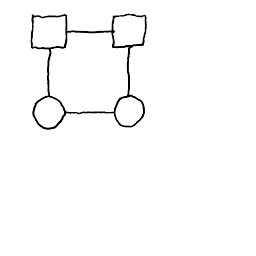
\includegraphics[width = 5cm]{../TikZ/drawings/expert-12.png}&
            \includegraphics[width = 5cm]{../TikZ/drawings/expert-12-parses/0.png}&
    
        \begin{minipage}{10cm}
        \begin{verbatim}
line(2,6,5,6,
arrow = False,solid = True);
reflect(reflect(x = 7)){
circle(6,1);
line(2,1,5,1,
arrow = False,solid = True);
line(1,2,1,5,
arrow = False,solid = True);
rectangle(5,5,7,7)
}
        \end{verbatim}
\end{minipage}

    \end{tabular}        
            \\

            \begin{tabular}{lll}
    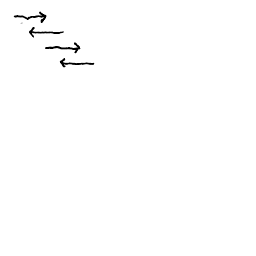
\includegraphics[width = 5cm]{../TikZ/drawings/expert-13.png}&
            \includegraphics[width = 5cm]{../TikZ/drawings/expert-13-parses/0.png}&
    
        \begin{minipage}{10cm}
        \begin{verbatim}
line(2,1,4,1,
arrow = True,solid = True);
line(3,2,1,2,
arrow = True,solid = True);
line(5,0,3,0,
arrow = True,solid = True);
line(0,3,2,3,
arrow = True,solid = True)
        \end{verbatim}
\end{minipage}

    \end{tabular}        
            \\

            \begin{tabular}{lll}
    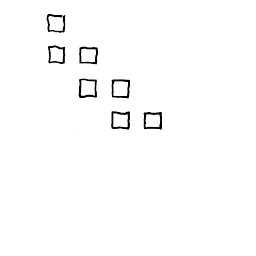
\includegraphics[width = 5cm]{../TikZ/drawings/expert-14.png}&
            \includegraphics[width = 5cm]{../TikZ/drawings/expert-14-parses/0.png}&
    
        \begin{minipage}{10cm}
        \begin{verbatim}
for (i < 4){
if (i > 0){
rectangle(-2*i + 6,2*i + -2,-2*i + 7,2*i + -1)
}
rectangle(-2*i + 6,2*i,-2*i + 7,2*i + 1)
}
        \end{verbatim}
\end{minipage}

    \end{tabular}        
            \\

            \begin{tabular}{lll}
    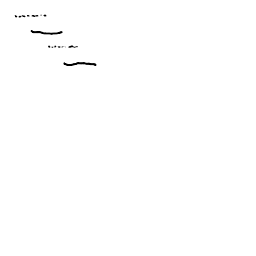
\includegraphics[width = 5cm]{../TikZ/drawings/expert-15.png}&
            \includegraphics[width = 5cm]{../TikZ/drawings/expert-15-parses/0.png}&
    
        \begin{minipage}{10cm}
        \begin{verbatim}
line(0,3,2,3,
arrow = False,solid = False);
line(2,1,4,1,
arrow = False,solid = False);
line(1,2,3,2,
arrow = False,solid = True);
line(3,0,5,0,
arrow = False,solid = True)
        \end{verbatim}
\end{minipage}

    \end{tabular}        
            \\

            \begin{tabular}{lll}
    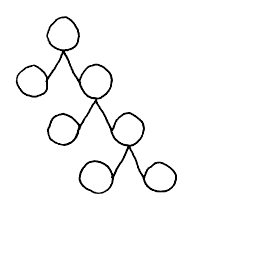
\includegraphics[width = 5cm]{../TikZ/drawings/expert-16.png}&
            \includegraphics[width = 5cm]{../TikZ/drawings/expert-16-parses/0.png}&
    
        \begin{minipage}{10cm}
        \begin{verbatim}
for (i < 4){
if (i > 0){
circle(-2*i + 7,3*i + -2);
line(-2*i + 9,3*i,-2*i + 10,3*i + -2,
arrow = False,solid = True);
line(-2*i + 8,3*i + -2,-2*i + 9,3*i,
arrow = False,solid = True)
}
circle(-2*i + 9,3*i + 1)
}
        \end{verbatim}
\end{minipage}

    \end{tabular}        
            \\

            \begin{tabular}{lll}
    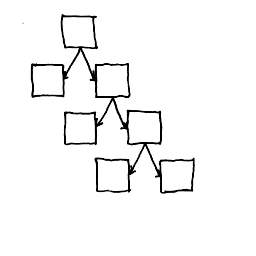
\includegraphics[width = 5cm]{../TikZ/drawings/expert-17.png}&
            \includegraphics[width = 5cm]{../TikZ/drawings/expert-17-parses/0.png}&
    
        \begin{minipage}{10cm}
        \begin{verbatim}
for (i < 4){
if (i > 0){
line(2*i + 1,-3*i + 12,2*i,-3*i + 10,
arrow = True,solid = True);
line(2*i + 1,-3*i + 12,2*i + 2,-3*i + 10,
arrow = True,solid = True);
rectangle(2*i + -2,-3*i + 9,2*i,-3*i + 11)
}
rectangle(2*i + 2,-3*i + 9,2*i + 4,-3*i + 11)
}
        \end{verbatim}
\end{minipage}

    \end{tabular}        
            \\

            \begin{tabular}{lll}
    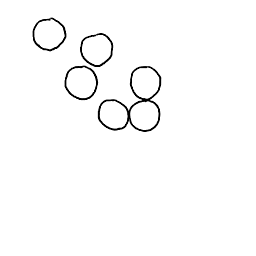
\includegraphics[width = 5cm]{../TikZ/drawings/expert-18.png}&
            \includegraphics[width = 5cm]{../TikZ/drawings/expert-18-parses/0.png}&
    
        \begin{minipage}{10cm}
        \begin{verbatim}
circle(5,1);
for (i < 3){
if (i > 0){
circle(7,2*i + -1);
circle(i + 2,2*i + 1)
}
circle(1,6)
}
        \end{verbatim}
\end{minipage}

    \end{tabular}        
            \\

            \begin{tabular}{lll}
    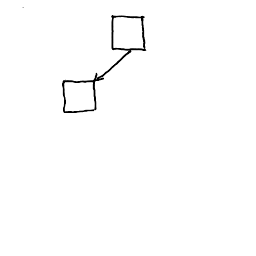
\includegraphics[width = 5cm]{../TikZ/drawings/expert-19.png}&
            \includegraphics[width = 5cm]{../TikZ/drawings/expert-19-parses/0.png}&
    
        \begin{minipage}{10cm}
        \begin{verbatim}
line(4,4,2,2,
arrow = True,solid = True);
rectangle(3,4,5,6);
rectangle(0,0,2,2)
        \end{verbatim}
\end{minipage}

    \end{tabular}        
            \\

            \begin{tabular}{lll}
    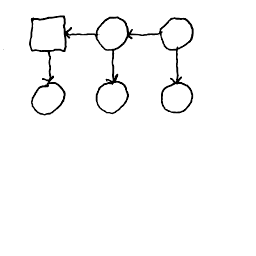
\includegraphics[width = 5cm]{../TikZ/drawings/expert-20.png}&
            \includegraphics[width = 5cm]{../TikZ/drawings/expert-20-parses/0.png}&
    
        \begin{minipage}{10cm}
        \begin{verbatim}
rectangle(0,4,2,6);
for (i < 3){
if (i > 0){
line(-4*i + 12,5,-4*i + 10,5,
arrow = True,solid = True);
for (j < i + 1){
circle(-4*j + 9,-4*i + 9)
}
}
line(-4*i + 9,4,-4*i + 9,2,
arrow = True,solid = True)
}
        \end{verbatim}
\end{minipage}

    \end{tabular}        
            \\

            \begin{tabular}{lll}
    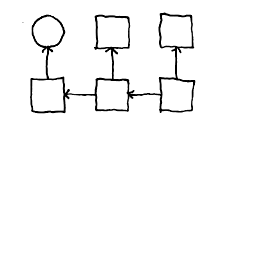
\includegraphics[width = 5cm]{../TikZ/drawings/expert-21.png}&
            \includegraphics[width = 5cm]{../TikZ/drawings/expert-21-parses/0.png}&
    
        \begin{minipage}{10cm}
        \begin{verbatim}
Solver timeout
        \end{verbatim}
\end{minipage}

    \end{tabular}        
            \\

            \begin{tabular}{lll}
    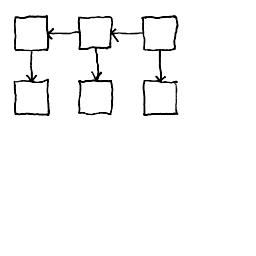
\includegraphics[width = 5cm]{../TikZ/drawings/expert-22.png}&
            \includegraphics[width = 5cm]{../TikZ/drawings/expert-22-parses/0.png}&
    
        \begin{minipage}{10cm}
        \begin{verbatim}
for (i < 3){
line(-4*i + 9,4,-4*i + 9,2,
arrow = True,solid = True);
for (j < 2){
line(-4*j + 8,5,-4*j + 6,5,
arrow = True,solid = True);
rectangle(-4*i + 8,4*j,-4*i + 10,4*j + 2)
}
}
        \end{verbatim}
\end{minipage}

    \end{tabular}        
            \\

            \begin{tabular}{lll}
    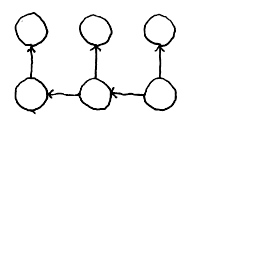
\includegraphics[width = 5cm]{../TikZ/drawings/expert-23.png}&
            \includegraphics[width = 5cm]{../TikZ/drawings/expert-23-parses/0.png}&
    
        \begin{minipage}{10cm}
        \begin{verbatim}
for (i < 3){
if (i > 0){
line(-4*i + 12,1,-4*i + 10,1,
arrow = True,solid = True)
}
circle(-4*i + 9,1);
circle(-4*i + 9,5);
line(-4*i + 9,2,-4*i + 9,4,
arrow = True,solid = True)
}
        \end{verbatim}
\end{minipage}

    \end{tabular}        
            \\

            \begin{tabular}{lll}
    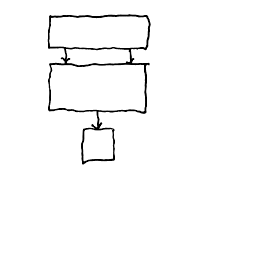
\includegraphics[width = 5cm]{../TikZ/drawings/expert-24.png}&
            \includegraphics[width = 5cm]{../TikZ/drawings/expert-24-parses/0.png}&
    
        \begin{minipage}{10cm}
        \begin{verbatim}
reflect(reflect(x = 6)){
for (i < 3){
if (i > 0){
line(-2*i + 7,-4*i + 11,-2*i + 7,-4*i + 10,
arrow = True,solid = True);
rectangle(0,-4*i + 11,6,-3*i + 12)
}
rectangle(2,0,4,2)
}
}
        \end{verbatim}
\end{minipage}

    \end{tabular}        
            \\

            \begin{tabular}{lll}
    \includegraphics[width = 5cm]{../TikZ/drawings/expert-25.png}&
            \includegraphics[width = 5cm]{../TikZ/drawings/expert-25-parses/0.png}&
    
        \begin{minipage}{10cm}
        \begin{verbatim}
for (i < 3){
if (i > 0){
line(3*i,1,3*i + -1,1,
arrow = True,solid = True)
}
rectangle(3*i,0,3*i + 2,2)
}
        \end{verbatim}
\end{minipage}

    \end{tabular}        
            \\

            \begin{tabular}{lll}
    \includegraphics[width = 5cm]{../TikZ/drawings/expert-26.png}&
            \includegraphics[width = 5cm]{../TikZ/drawings/expert-26-parses/0.png}&
    
        \begin{minipage}{10cm}
        \begin{verbatim}
line(1,3,1,4,
arrow = False,solid = True);
for (i < 3){
if (i > 0){
line(1,-5*i + 13,1,-4*i + 10,
arrow = True,solid = True)
}
circle(1,-4*i + 9)
}
        \end{verbatim}
\end{minipage}

    \end{tabular}        
            \\

            \begin{tabular}{lll}
    \includegraphics[width = 5cm]{../TikZ/drawings/expert-27.png}&
            \includegraphics[width = 5cm]{../TikZ/drawings/expert-27-parses/0.png}&
    
        \begin{minipage}{10cm}
        \begin{verbatim}
reflect(reflect(x = 2)){
line(0,1,1,2,
arrow = False,solid = True);
line(1,0,2,1,
arrow = False,solid = True)
}
        \end{verbatim}
\end{minipage}

    \end{tabular}        
            \\

            \begin{tabular}{lll}
    \includegraphics[width = 5cm]{../TikZ/drawings/expert-28.png}&
            \includegraphics[width = 5cm]{../TikZ/drawings/expert-28-parses/0.png}&
    
        \begin{minipage}{10cm}
        \begin{verbatim}
line(0,0,0,2,
arrow = False,solid = True);
line(0,2,2,2,
arrow = False,solid = True)
        \end{verbatim}
\end{minipage}

    \end{tabular}        
            \\

            \begin{tabular}{lll}
    \includegraphics[width = 5cm]{../TikZ/drawings/expert-29.png}&
            \includegraphics[width = 5cm]{../TikZ/drawings/expert-29-parses/0.png}&
    
        \begin{minipage}{10cm}
        \begin{verbatim}
for (i < 3){
line(i,-1*i + 6,2*i + 2,-1*i + 6,
arrow = False,solid = True);
line(i,-2*i + 4,i,-1*i + 6,
arrow = False,solid = True)
}
        \end{verbatim}
\end{minipage}

    \end{tabular}        
            \\

            \begin{tabular}{lll}
    \includegraphics[width = 5cm]{../TikZ/drawings/expert-30.png}&
            \includegraphics[width = 5cm]{../TikZ/drawings/expert-30-parses/0.png}&
    
        \begin{minipage}{10cm}
        \begin{verbatim}
for (i < 3){
if (i > 0){
circle(1,-3*i + 7);
circle(5,-2*i + 6);
rectangle(0,-3*i + 6,2,-3*i + 8)
}
rectangle(4,1,6,5)
}
        \end{verbatim}
\end{minipage}

    \end{tabular}        
            \\

            \begin{tabular}{lll}
    \includegraphics[width = 5cm]{../TikZ/drawings/expert-31.png}&
            \includegraphics[width = 5cm]{../TikZ/drawings/expert-31-parses/0.png}&
    
        \begin{minipage}{10cm}
        \begin{verbatim}
for (i < 3){
rectangle(3*i,-2*i + 4,3*i + 2,6);
for (j < i + 1){
circle(3*i + 1,-2*j + 5)
}
}
        \end{verbatim}
\end{minipage}

    \end{tabular}        
            \\

            \begin{tabular}{lll}
    \includegraphics[width = 5cm]{../TikZ/drawings/expert-32.png}&
            \includegraphics[width = 5cm]{../TikZ/drawings/expert-32-parses/0.png}&
    
        \begin{minipage}{10cm}
        \begin{verbatim}
circle(5,5);
line(2,5,4,5,
arrow = False,solid = True);
rectangle(0,0,5,3);
rectangle(0,4,2,6)
        \end{verbatim}
\end{minipage}

    \end{tabular}        
            \\

            \begin{tabular}{lll}
    \includegraphics[width = 5cm]{../TikZ/drawings/expert-33.png}&
            \includegraphics[width = 5cm]{../TikZ/drawings/expert-33-parses/0.png}&
    
        \begin{minipage}{10cm}
        \begin{verbatim}
line(0,0,6,0,
arrow = False,solid = False);
reflect(reflect(x = 6)){
line(6,0,6,3,
arrow = False,solid = True);
line(0,3,6,3,
arrow = False,solid = False)
}
        \end{verbatim}
\end{minipage}

    \end{tabular}        
            \\

            \begin{tabular}{lll}
    \includegraphics[width = 5cm]{../TikZ/drawings/expert-34.png}&
            \includegraphics[width = 5cm]{../TikZ/drawings/expert-34-parses/0.png}&
    
        \begin{minipage}{10cm}
        \begin{verbatim}
Solver timeout
        \end{verbatim}
\end{minipage}

    \end{tabular}        
            \\

            \begin{tabular}{lll}
    \includegraphics[width = 5cm]{../TikZ/drawings/expert-35.png}&
            \includegraphics[width = 5cm]{../TikZ/drawings/expert-35-parses/0.png}&
    
        \begin{minipage}{10cm}
        \begin{verbatim}
for (i < 3){
if (i > 0){
circle(-5*i + 11,1);
line(-1*i + 3,-1*i + 7,-5*i + 11,2,
arrow = True,solid = True)
}
circle(1,6)
}
        \end{verbatim}
\end{minipage}

    \end{tabular}        
            \\

            \begin{tabular}{lll}
    \includegraphics[width = 5cm]{../TikZ/drawings/expert-36.png}&
            \includegraphics[width = 5cm]{../TikZ/drawings/expert-36-parses/0.png}&
    
        \begin{minipage}{10cm}
        \begin{verbatim}
Solver timeout
        \end{verbatim}
\end{minipage}

    \end{tabular}        
            \\

            \begin{tabular}{lll}
    \includegraphics[width = 5cm]{../TikZ/drawings/expert-37.png}&
            \includegraphics[width = 5cm]{../TikZ/drawings/expert-37-parses/0.png}&
    
        \begin{minipage}{10cm}
        \begin{verbatim}
for (i < 3){
if (i > 0){
line(4*i + -3,-5*i + 12,2*i + 1,5,
arrow = False,solid = True);
rectangle(4*i + -4,-5*i + 10,6,-7*i + 16)
}
circle(1,8)
}
        \end{verbatim}
\end{minipage}

    \end{tabular}        
            \\

            \begin{tabular}{lll}
    \includegraphics[width = 5cm]{../TikZ/drawings/expert-38.png}&
            \includegraphics[width = 5cm]{../TikZ/drawings/expert-38-parses/0.png}&
    
        \begin{minipage}{10cm}
        \begin{verbatim}
Solver timeout
        \end{verbatim}
\end{minipage}

    \end{tabular}        
            \\

            \begin{tabular}{lll}
    \includegraphics[width = 5cm]{../TikZ/drawings/expert-39.png}&
            \includegraphics[width = 5cm]{../TikZ/drawings/expert-39-parses/0.png}&
    
        \begin{minipage}{10cm}
        \begin{verbatim}
Solver timeout
        \end{verbatim}
\end{minipage}

    \end{tabular}        
            \\

            \begin{tabular}{lll}
    \includegraphics[width = 5cm]{../TikZ/drawings/expert-40.png}&
            \includegraphics[width = 5cm]{../TikZ/drawings/expert-40-parses/0.png}&
    
        \begin{minipage}{10cm}
        \begin{verbatim}
for (i < 3){
circle(-3*i + 7,1)
}
        \end{verbatim}
\end{minipage}

    \end{tabular}        
            \\

            \begin{tabular}{lll}
    \includegraphics[width = 5cm]{../TikZ/drawings/expert-41.png}&
            \includegraphics[width = 5cm]{../TikZ/drawings/expert-41-parses/0.png}&
    
        \begin{minipage}{10cm}
        \begin{verbatim}
for (i < 3){
rectangle(-2*i + 4,0,-2*i + 5,6)
}
        \end{verbatim}
\end{minipage}

    \end{tabular}        
            \\

            \begin{tabular}{lll}
    \includegraphics[width = 5cm]{../TikZ/drawings/expert-42.png}&
            \includegraphics[width = 5cm]{../TikZ/drawings/expert-42-parses/0.png}&
    
        \begin{minipage}{10cm}
        \begin{verbatim}
line(4,0,4,1,
arrow = False,solid = False);
line(0,0,0,5,
arrow = False,solid = False);
line(4,1,4,5,
arrow = False,solid = False)
        \end{verbatim}
\end{minipage}

    \end{tabular}        
            \\

            \begin{tabular}{lll}
    \includegraphics[width = 5cm]{../TikZ/drawings/expert-43.png}&
            \includegraphics[width = 5cm]{../TikZ/drawings/expert-43-parses/0.png}&
    
        \begin{minipage}{10cm}
        \begin{verbatim}
line(4,0,4,5,
arrow = False,solid = True);
line(0,0,0,5,
arrow = False,solid = True)
        \end{verbatim}
\end{minipage}

    \end{tabular}        
            \\

            \begin{tabular}{lll}
    \includegraphics[width = 5cm]{../TikZ/drawings/expert-44.png}&
            \includegraphics[width = 5cm]{../TikZ/drawings/expert-44-parses/0.png}&
    
        \begin{minipage}{10cm}
        \begin{verbatim}
reflect(reflect(x = 12)){
circle(4,1);
line(9,1,10,1,
arrow = False,solid = True);
rectangle(0,0,2,2)
}
        \end{verbatim}
\end{minipage}

    \end{tabular}        
            \\

            \begin{tabular}{lll}
    \includegraphics[width = 5cm]{../TikZ/drawings/expert-45.png}&
            \includegraphics[width = 5cm]{../TikZ/drawings/expert-45-parses/0.png}&
    
        \begin{minipage}{10cm}
        \begin{verbatim}
rectangle(0,4,4,8);
reflect(reflect(y = 12)){
circle(7,6);
line(2,2,2,4,
arrow = True,solid = True);
line(4,6,6,6,
arrow = True,solid = True);
rectangle(1,10,3,12)
}
        \end{verbatim}
\end{minipage}

    \end{tabular}        
            \\

            \begin{tabular}{lll}
    \includegraphics[width = 5cm]{../TikZ/drawings/expert-46.png}&
            \includegraphics[width = 5cm]{../TikZ/drawings/expert-46-parses/0.png}&
    
        \begin{minipage}{10cm}
        \begin{verbatim}
reflect(reflect(y = 9)){
line(3,8,6,8,
arrow = False,solid = True);
reflect(reflect(x = 9)){
circle(1,8);
line(1,3,1,6,
arrow = False,solid = True)
}
}
        \end{verbatim}
\end{minipage}

    \end{tabular}        
            \\

            \begin{tabular}{lll}
    \includegraphics[width = 5cm]{../TikZ/drawings/expert-47.png}&
            \includegraphics[width = 5cm]{../TikZ/drawings/expert-47-parses/0.png}&
    
        \begin{minipage}{10cm}
        \begin{verbatim}
reflect(reflect(y = 11)){
rectangle(4,9,7,10);
reflect(reflect(x = 11)){
rectangle(1,4,2,7);
rectangle(8,8,11,11)
}
}
        \end{verbatim}
\end{minipage}

    \end{tabular}        
            \\

            \begin{tabular}{lll}
    \includegraphics[width = 5cm]{../TikZ/drawings/expert-48.png}&
            \includegraphics[width = 5cm]{../TikZ/drawings/expert-48-parses/0.png}&
    
        \begin{minipage}{10cm}
        \begin{verbatim}
for (i < 4){
line(i,-1*i + 5,i + 2,-1*i + 5,
arrow = False,solid = True);
line(i + 2,-1*i + 3,i + 4,-1*i + 3,
arrow = False,solid = True)
}
        \end{verbatim}
\end{minipage}

    \end{tabular}        
            \\

            \begin{tabular}{lll}
    \includegraphics[width = 5cm]{../TikZ/drawings/expert-49.png}&
            \includegraphics[width = 5cm]{../TikZ/drawings/expert-49-parses/0.png}&
    
        \begin{minipage}{10cm}
        \begin{verbatim}
for (i < 3){
if (i > 0){
rectangle(3*i + 1,-1*i + 2,3*i + 3,2);
rectangle(0,7*i + -7,3,7*i + -4)
}
rectangle(1,4,2,6)
}
        \end{verbatim}
\end{minipage}

    \end{tabular}        
            \\

            \begin{tabular}{lll}
    \includegraphics[width = 5cm]{../TikZ/drawings/expert-50.png}&
            \includegraphics[width = 5cm]{../TikZ/drawings/expert-50-parses/0.png}&
    
        \begin{minipage}{10cm}
        \begin{verbatim}
Solver timeout
        \end{verbatim}
\end{minipage}

    \end{tabular}        
            \\

            \begin{tabular}{lll}
    \includegraphics[width = 5cm]{../TikZ/drawings/expert-51.png}&
            \includegraphics[width = 5cm]{../TikZ/drawings/expert-51-parses/0.png}&
    
        \begin{minipage}{10cm}
        \begin{verbatim}
for (i < 3){
rectangle(-2*i + 4,-2*i + 4,-2*i + 7,-2*i + 5)
}
        \end{verbatim}
\end{minipage}

    \end{tabular}        
            \\

            \begin{tabular}{lll}
    \includegraphics[width = 5cm]{../TikZ/drawings/expert-52.png}&
            \includegraphics[width = 5cm]{../TikZ/drawings/expert-52-parses/0.png}&
    
        \begin{minipage}{10cm}
        \begin{verbatim}
circle(4,10);
for (i < 3){
circle(-3*i + 7,5);
circle(-3*i + 7,1);
line(-3*i + 7,4,-3*i + 7,2,
arrow = True,solid = True);
line(4,9,-3*i + 7,6,
arrow = True,solid = True)
}
        \end{verbatim}
\end{minipage}

    \end{tabular}        
            \\

            \begin{tabular}{lll}
    \includegraphics[width = 5cm]{../TikZ/drawings/expert-53.png}&
            \includegraphics[width = 5cm]{../TikZ/drawings/expert-53-parses/0.png}&
    
        \begin{minipage}{10cm}
        \begin{verbatim}
line(2,8,2,6,
arrow = True,solid = True);
line(6,8,6,4,
arrow = True,solid = True);
line(4,8,4,0,
arrow = True,solid = True);
line(0,8,8,8,
arrow = False,solid = True)
        \end{verbatim}
\end{minipage}

    \end{tabular}        
            \\

            \begin{tabular}{lll}
    \includegraphics[width = 5cm]{../TikZ/drawings/expert-54.png}&
            \includegraphics[width = 5cm]{../TikZ/drawings/expert-54-parses/0.png}&
    
        \begin{minipage}{10cm}
        \begin{verbatim}
line(2,3,2,5,
arrow = False,solid = True);
rectangle(1,1,3,3);
rectangle(1,5,3,7);
rectangle(0,0,4,8)
        \end{verbatim}
\end{minipage}

    \end{tabular}        
            \\

            \begin{tabular}{lll}
    \includegraphics[width = 5cm]{../TikZ/drawings/expert-55.png}&
            \includegraphics[width = 5cm]{../TikZ/drawings/expert-55-parses/0.png}&
    
        \begin{minipage}{10cm}
        \begin{verbatim}
circle(1,5);
line(1,4,1,2,
arrow = True,solid = True);
rectangle(0,0,2,2)
        \end{verbatim}
\end{minipage}

    \end{tabular}        
            \\

            \begin{tabular}{lll}
    \includegraphics[width = 5cm]{../TikZ/drawings/expert-56.png}&
            \includegraphics[width = 5cm]{../TikZ/drawings/expert-56-parses/0.png}&
    
        \begin{minipage}{10cm}
        \begin{verbatim}
Solver timeout
        \end{verbatim}
\end{minipage}

    \end{tabular}        
            \\

            \begin{tabular}{lll}
    \includegraphics[width = 5cm]{../TikZ/drawings/expert-57.png}&
            \includegraphics[width = 5cm]{../TikZ/drawings/expert-57-parses/0.png}&
    
        \begin{minipage}{10cm}
        \begin{verbatim}
for (i < 3){
for (j < 3){
circle(-4*j + 9,-3*i + 7)
}
}
        \end{verbatim}
\end{minipage}

    \end{tabular}        
            \\

            \begin{tabular}{lll}
    \includegraphics[width = 5cm]{../TikZ/drawings/expert-58.png}&
            \includegraphics[width = 5cm]{../TikZ/drawings/expert-58-parses/0.png}&
    
        \begin{minipage}{10cm}
        \begin{verbatim}
for (i < 3){
if (i > 0){
line(8,0,8*i + -8,7*i + -7,
arrow = True,solid = True)
}
rectangle(2*i + 2,0,2*i + 3,i + 3)
}
        \end{verbatim}
\end{minipage}

    \end{tabular}        
            \\

            \begin{tabular}{lll}
    \includegraphics[width = 5cm]{../TikZ/drawings/expert-59.png}&
            \includegraphics[width = 5cm]{../TikZ/drawings/expert-59-parses/0.png}&
    
        \begin{minipage}{10cm}
        \begin{verbatim}
line(4,0,0,0,
arrow = False,solid = False)
        \end{verbatim}
\end{minipage}

    \end{tabular}        
            \\

            \begin{tabular}{lll}
    \includegraphics[width = 5cm]{../TikZ/drawings/expert-60.png}&
            \includegraphics[width = 5cm]{../TikZ/drawings/expert-60-parses/0.png}&
    
        \begin{minipage}{10cm}
        \begin{verbatim}
Solver timeout
        \end{verbatim}
\end{minipage}

    \end{tabular}        
            \\

            \begin{tabular}{lll}
    \includegraphics[width = 5cm]{../TikZ/drawings/expert-61.png}&
            \includegraphics[width = 5cm]{../TikZ/drawings/expert-61-parses/0.png}&
    
        \begin{minipage}{10cm}
        \begin{verbatim}
circle(2,1);
circle(6,1);
line(5,1,3,1,
arrow = True,solid = True);
rectangle(0,0,7,2)
        \end{verbatim}
\end{minipage}

    \end{tabular}        
            \\

            \begin{tabular}{lll}
    \includegraphics[width = 5cm]{../TikZ/drawings/expert-62.png}&
            \includegraphics[width = 5cm]{../TikZ/drawings/expert-62-parses/0.png}&
    
        \begin{minipage}{10cm}
        \begin{verbatim}
rectangle(5,0,8,3);
rectangle(2,1,4,3);
rectangle(0,2,1,3)
        \end{verbatim}
\end{minipage}

    \end{tabular}        
            \\

            \begin{tabular}{lll}
    \includegraphics[width = 5cm]{../TikZ/drawings/expert-63.png}&
            \includegraphics[width = 5cm]{../TikZ/drawings/expert-63-parses/0.png}&
    
        \begin{minipage}{10cm}
        \begin{verbatim}
for (i < 3){
rectangle(-1*i + 2,-1*i + 2,i + 3,i + 3)
}
        \end{verbatim}
\end{minipage}

    \end{tabular}        
            \\

            \begin{tabular}{lll}
    \includegraphics[width = 5cm]{../TikZ/drawings/expert-64.png}&
            \includegraphics[width = 5cm]{../TikZ/drawings/expert-64-parses/0.png}&
    
        \begin{minipage}{10cm}
        \begin{verbatim}
reflect(reflect(x = 6)){
line(5,2,5,4,
arrow = False,solid = True);
reflect(reflect(y = 6)){
line(2,1,4,1,
arrow = False,solid = True);
rectangle(4,4,6,6)
}
}
        \end{verbatim}
\end{minipage}

    \end{tabular}        
            \\

            \begin{tabular}{lll}
    \includegraphics[width = 5cm]{../TikZ/drawings/expert-65.png}&
            \includegraphics[width = 5cm]{../TikZ/drawings/expert-65-parses/0.png}&
    
        \begin{minipage}{10cm}
        \begin{verbatim}
reflect(reflect(y = 6)){
line(2,5,4,5,
arrow = False,solid = True);
reflect(reflect(x = 6)){
circle(5,5);
line(1,2,1,4,
arrow = False,solid = True)
}
}
        \end{verbatim}
\end{minipage}

    \end{tabular}        
            \\

            \begin{tabular}{lll}
    \includegraphics[width = 5cm]{../TikZ/drawings/expert-66.png}&
            \includegraphics[width = 5cm]{../TikZ/drawings/expert-66-parses/0.png}&
    
        \begin{minipage}{10cm}
        \begin{verbatim}
for (i < 3){
line(i,-1*i + 2,-1*i + 7,-1*i + 2,
arrow = False,solid = True)
}
        \end{verbatim}
\end{minipage}

    \end{tabular}        
            \\

            \begin{tabular}{lll}
    \includegraphics[width = 5cm]{../TikZ/drawings/expert-67.png}&
            \includegraphics[width = 5cm]{../TikZ/drawings/expert-67-parses/0.png}&
    
        \begin{minipage}{10cm}
        \begin{verbatim}
line(1,4,5,0,
arrow = False,solid = True);
line(1,5,5,1,
arrow = False,solid = True);
rectangle(5,0,6,1);
rectangle(0,4,1,5)
        \end{verbatim}
\end{minipage}

    \end{tabular}        
            \\

            \begin{tabular}{lll}
    \includegraphics[width = 5cm]{../TikZ/drawings/expert-68.png}&
            \includegraphics[width = 5cm]{../TikZ/drawings/expert-68-parses/0.png}&
    
        \begin{minipage}{10cm}
        \begin{verbatim}
for (i < 3){
circle(4*i + 1,1);
rectangle(4*i,0,4*i + 2,2)
}
        \end{verbatim}
\end{minipage}

    \end{tabular}        
            \\

            \begin{tabular}{lll}
    \includegraphics[width = 5cm]{../TikZ/drawings/expert-69.png}&
            \includegraphics[width = 5cm]{../TikZ/drawings/expert-69-parses/0.png}&
    
        \begin{minipage}{10cm}
        \begin{verbatim}
reflect(reflect(x = 5)){
circle(1,1);
line(4,4,4,2,
arrow = True,solid = True);
rectangle(0,4,5,6)
}
        \end{verbatim}
\end{minipage}

    \end{tabular}        
            \\

            \begin{tabular}{lll}
    \includegraphics[width = 5cm]{../TikZ/drawings/expert-70.png}&
            \includegraphics[width = 5cm]{../TikZ/drawings/expert-70-parses/0.png}&
    
        \begin{minipage}{10cm}
        \begin{verbatim}
Solver timeout
        \end{verbatim}
\end{minipage}

    \end{tabular}        
            \\

            \begin{tabular}{lll}
    \includegraphics[width = 5cm]{../TikZ/drawings/expert-71.png}&
            Sampled no finished traces.&
    
        \begin{minipage}{10cm}
        \begin{verbatim}
Solver timeout
        \end{verbatim}
\end{minipage}

    \end{tabular}        
            \\

            \begin{tabular}{lll}
    \includegraphics[width = 5cm]{../TikZ/drawings/expert-72.png}&
            \includegraphics[width = 5cm]{../TikZ/drawings/expert-72-parses/0.png}&
    
        \begin{minipage}{10cm}
        \begin{verbatim}
reflect(reflect(y = 8)){
for (i < 3){
if (i > 0){
rectangle(3*i + -1,2,3*i,3)
}
circle(3*i + 1,3*i + 1)
}
}
        \end{verbatim}
\end{minipage}

    \end{tabular}        
            \\

            \begin{tabular}{lll}
    \includegraphics[width = 5cm]{../TikZ/drawings/expert-73.png}&
            Sampled no finished traces.&
    
        \begin{minipage}{10cm}
        \begin{verbatim}
Solver timeout
        \end{verbatim}
\end{minipage}

    \end{tabular}        
            \\

            \begin{tabular}{lll}
    \includegraphics[width = 5cm]{../TikZ/drawings/expert-74.png}&
            \includegraphics[width = 5cm]{../TikZ/drawings/expert-74-parses/0.png}&
    
        \begin{minipage}{10cm}
        \begin{verbatim}
for (i < 3){
if (i > 0){
rectangle(-2*i + 4,-2*i + 4,2*i + 2,2*i + 2)
}
for (j < 3){
circle(-2*i + 5,2*j + 1)
}
}
        \end{verbatim}
\end{minipage}

    \end{tabular}        
            \\

            \begin{tabular}{lll}
    \includegraphics[width = 5cm]{../TikZ/drawings/expert-75.png}&
            \includegraphics[width = 5cm]{../TikZ/drawings/expert-75-parses/0.png}&
    
        \begin{minipage}{10cm}
        \begin{verbatim}
for (i < 4){
line(-4*i + 13,4,-4*i + 13,2,
arrow = True,solid = True);
for (j < 3){
if (j > 0){
circle(-4*i + 13,4*j + -3)
}
line(-4*j + 10,5,-4*j + 12,5,
arrow = True,solid = True)
}
}
        \end{verbatim}
\end{minipage}

    \end{tabular}        
            \\

            \begin{tabular}{lll}
    \includegraphics[width = 5cm]{../TikZ/drawings/expert-76.png}&
            \includegraphics[width = 5cm]{../TikZ/drawings/expert-76-parses/0.png}&
    
        \begin{minipage}{10cm}
        \begin{verbatim}
circle(4,1);
reflect(reflect(x = 8)){
circle(1,8);
line(4,5,8,2,
arrow = False,solid = True);
line(4,5,4,10,
arrow = False,solid = True)
}
        \end{verbatim}
\end{minipage}

    \end{tabular}        
            \\

            \begin{tabular}{lll}
    \includegraphics[width = 5cm]{../TikZ/drawings/expert-77.png}&
            \includegraphics[width = 5cm]{../TikZ/drawings/expert-77-parses/0.png}&
    
        \begin{minipage}{10cm}
        \begin{verbatim}
Solver timeout
        \end{verbatim}
\end{minipage}

    \end{tabular}        
            \\

            \begin{tabular}{lll}
    \includegraphics[width = 5cm]{../TikZ/drawings/expert-78.png}&
            \includegraphics[width = 5cm]{../TikZ/drawings/expert-78-parses/0.png}&
    
        \begin{minipage}{10cm}
        \begin{verbatim}
line(0,6,12,6,
arrow = False,solid = True);
line(6,6,6,5,
arrow = True,solid = True);
line(8,3,7,4,
arrow = True,solid = True);
line(3,2,5,4,
arrow = True,solid = True);
reflect(reflect(x = 12)){
line(4,0,12,8,
arrow = False,solid = True)
}
        \end{verbatim}
\end{minipage}

    \end{tabular}        
            \\

            \begin{tabular}{lll}
    \includegraphics[width = 5cm]{../TikZ/drawings/expert-79.png}&
            \includegraphics[width = 5cm]{../TikZ/drawings/expert-79-parses/0.png}&
    
        \begin{minipage}{10cm}
        \begin{verbatim}
Solver timeout
        \end{verbatim}
\end{minipage}

    \end{tabular}        
            \\

            \begin{tabular}{lll}
    \includegraphics[width = 5cm]{../TikZ/drawings/expert-80.png}&
            \includegraphics[width = 5cm]{../TikZ/drawings/expert-80-parses/0.png}&
    
        \begin{minipage}{10cm}
        \begin{verbatim}
Solver timeout
        \end{verbatim}
\end{minipage}

    \end{tabular}        
            \\

            \begin{tabular}{lll}
    \includegraphics[width = 5cm]{../TikZ/drawings/expert-81.png}&
            \includegraphics[width = 5cm]{../TikZ/drawings/expert-81-parses/0.png}&
    
        \begin{minipage}{10cm}
        \begin{verbatim}
circle(1,1);
circle(4,1);
rectangle(9,0,11,2);
rectangle(6,0,8,2)
        \end{verbatim}
\end{minipage}

    \end{tabular}        
            \\

            \begin{tabular}{lll}
    \includegraphics[width = 5cm]{../TikZ/drawings/expert-82.png}&
            \includegraphics[width = 5cm]{../TikZ/drawings/expert-82-parses/0.png}&
    
        \begin{minipage}{10cm}
        \begin{verbatim}
Solver timeout
        \end{verbatim}
\end{minipage}

    \end{tabular}        
            \\

            \begin{tabular}{lll}
    \includegraphics[width = 5cm]{../TikZ/drawings/expert-83.png}&
            \includegraphics[width = 5cm]{../TikZ/drawings/expert-83-parses/0.png}&
    
        \begin{minipage}{10cm}
        \begin{verbatim}
Solver timeout
        \end{verbatim}
\end{minipage}

    \end{tabular}        
            \\

            \begin{tabular}{lll}
    \includegraphics[width = 5cm]{../TikZ/drawings/expert-84.png}&
            \includegraphics[width = 5cm]{../TikZ/drawings/expert-84-parses/0.png}&
    
        \begin{minipage}{10cm}
        \begin{verbatim}
Solver timeout
        \end{verbatim}
\end{minipage}

    \end{tabular}        
            \\

            \begin{tabular}{lll}
    \includegraphics[width = 5cm]{../TikZ/drawings/expert-85.png}&
            \includegraphics[width = 5cm]{../TikZ/drawings/expert-85-parses/0.png}&
    
        \begin{minipage}{10cm}
        \begin{verbatim}
for (i < 4){
if (i > 0){
line(1,-3*i + 12,1,-3*i + 11,
arrow = True,solid = True)
}
circle(1,-3*i + 10)
}
        \end{verbatim}
\end{minipage}

    \end{tabular}        
            \\

            \begin{tabular}{lll}
    \includegraphics[width = 5cm]{../TikZ/drawings/expert-86.png}&
            \includegraphics[width = 5cm]{../TikZ/drawings/expert-86-parses/0.png}&
    
        \begin{minipage}{10cm}
        \begin{verbatim}
Solver timeout
        \end{verbatim}
\end{minipage}

    \end{tabular}        
            \\

            \begin{tabular}{lll}
    \includegraphics[width = 5cm]{../TikZ/drawings/expert-87.png}&
            \includegraphics[width = 5cm]{../TikZ/drawings/expert-87-parses/0.png}&
    
        \begin{minipage}{10cm}
        \begin{verbatim}
reflect(reflect(x = 8)){
rectangle(0,5,3,8);
rectangle(0,2,2,4);
rectangle(0,0,1,1)
}
        \end{verbatim}
\end{minipage}

    \end{tabular}        
            \\

            \begin{tabular}{lll}
    \includegraphics[width = 5cm]{../TikZ/drawings/expert-88.png}&
            \includegraphics[width = 5cm]{../TikZ/drawings/expert-88-parses/0.png}&
    
        \begin{minipage}{10cm}
        \begin{verbatim}
for (i < 3){
rectangle(-2*i + 4,-1*i + 2,i + 6,2*i + 3)
}
        \end{verbatim}
\end{minipage}

    \end{tabular}        
            \\

            \begin{tabular}{lll}
    \includegraphics[width = 5cm]{../TikZ/drawings/expert-89.png}&
            \includegraphics[width = 5cm]{../TikZ/drawings/expert-89-parses/0.png}&
    
        \begin{minipage}{10cm}
        \begin{verbatim}
Solver timeout
        \end{verbatim}
\end{minipage}

    \end{tabular}        
            \\

            \begin{tabular}{lll}
    \includegraphics[width = 5cm]{../TikZ/drawings/expert-90.png}&
            \includegraphics[width = 5cm]{../TikZ/drawings/expert-90-parses/0.png}&
    
        \begin{minipage}{10cm}
        \begin{verbatim}
line(6,6,6,3,
arrow = True,solid = True);
for (i < 3){
if (i > 0){
circle(-5*i + 16,7);
circle(-5*i + 11,5*i + -3);
line(-5*i + 15,7,-5*i + 12,7,
arrow = True,solid = True)
}
rectangle(4,0,8,9)
}
        \end{verbatim}
\end{minipage}

    \end{tabular}        
            \\

            \begin{tabular}{lll}
    \includegraphics[width = 5cm]{../TikZ/drawings/expert-91.png}&
            \includegraphics[width = 5cm]{../TikZ/drawings/expert-91-parses/0.png}&
    
        \begin{minipage}{10cm}
        \begin{verbatim}
reflect(reflect(x = 5)){
reflect(reflect(y = 5)){
line(5,3,5,5,
arrow = False,solid = True);
line(3,5,5,5,
arrow = False,solid = True)
}
}
        \end{verbatim}
\end{minipage}

    \end{tabular}        
            \\

            \begin{tabular}{lll}
    \includegraphics[width = 5cm]{../TikZ/drawings/expert-92.png}&
            \includegraphics[width = 5cm]{../TikZ/drawings/expert-92-parses/0.png}&
    
        \begin{minipage}{10cm}
        \begin{verbatim}
reflect(reflect(x = 14)){
for (i < 3){
circle(9,-4*i + 9);
line(10,-4*i + 9,12,-4*i + 9,
arrow = False,solid = True);
rectangle(0,-4*i + 8,2,-4*i + 10)
}
}
        \end{verbatim}
\end{minipage}

    \end{tabular}        
            \\

            \begin{tabular}{lll}
    \includegraphics[width = 5cm]{../TikZ/drawings/expert-93.png}&
            \includegraphics[width = 5cm]{../TikZ/drawings/expert-93-parses/0.png}&
    
        \begin{minipage}{10cm}
        \begin{verbatim}
reflect(reflect(x = 10)){
for (i < 3){
if (i > 0){
line(4*i + -3,4*i + -2,4*i + 1,4*i,
arrow = True,solid = True)
}
circle(4*i + 1,4*i + 1)
}
}
        \end{verbatim}
\end{minipage}

    \end{tabular}        
            \\

            \begin{tabular}{lll}
    \includegraphics[width = 5cm]{../TikZ/drawings/expert-94.png}&
            Sampled no finished traces.&
    
        \begin{minipage}{10cm}
        \begin{verbatim}
line(0,2,12,2,
arrow = False,solid = True);
line(6,2,6,3,
arrow = True,solid = True);
reflect(reflect(x = 12)){
line(0,0,9,9,
arrow = False,solid = True);
line(10,7,7,4,
arrow = True,solid = True)
}
        \end{verbatim}
\end{minipage}

    \end{tabular}        
            \\

            \begin{tabular}{lll}
    \includegraphics[width = 5cm]{../TikZ/drawings/expert-95.png}&
            \includegraphics[width = 5cm]{../TikZ/drawings/expert-95-parses/0.png}&
    
        \begin{minipage}{10cm}
        \begin{verbatim}
reflect(reflect(x = 8)){
circle(4,1);
for (i < 3){
if (i > 0){
circle(7,-5*i + 16);
line(-6*i + 13,10,7,7,
arrow = True,solid = True)
}
line(1,5,4,2,
arrow = True,solid = True)
}
}
        \end{verbatim}
\end{minipage}

    \end{tabular}        
            \\

            \begin{tabular}{lll}
    \includegraphics[width = 5cm]{../TikZ/drawings/expert-96.png}&
            \includegraphics[width = 5cm]{../TikZ/drawings/expert-96-parses/0.png}&
    
        \begin{minipage}{10cm}
        \begin{verbatim}
reflect(reflect(x = 10)){
circle(1,1);
for (i < 4){
circle(-2*i + 7,2*i + 3)
}
}
        \end{verbatim}
\end{minipage}

    \end{tabular}        
            \\

            \begin{tabular}{lll}
    \includegraphics[width = 5cm]{../TikZ/drawings/expert-97.png}&
            \includegraphics[width = 5cm]{../TikZ/drawings/expert-97-parses/0.png}&
    
        \begin{minipage}{10cm}
        \begin{verbatim}
reflect(reflect(x = 6)){
for (i < 3){
if (i > 0){
line(1,-4*i + 10,1,-4*i + 12,
arrow = False,solid = True)
}
circle(5,-4*i + 9);
line(2,-4*i + 9,4,-4*i + 9,
arrow = False,solid = True)
}
}
        \end{verbatim}
\end{minipage}

    \end{tabular}        
            \\

            \begin{tabular}{lll}
    \includegraphics[width = 5cm]{../TikZ/drawings/expert-98.png}&
            \includegraphics[width = 5cm]{../TikZ/drawings/expert-98-parses/0.png}&
    
        \begin{minipage}{10cm}
        \begin{verbatim}
rectangle(0,0,4,9);
for (i < 3){
if (i > 0){
circle(2,-4*i + 10);
line(2,-5*i + 15,2,-4*i + 11,
arrow = True,solid = True)
}
circle(2,11)
}
        \end{verbatim}
\end{minipage}

    \end{tabular}        
            \\

            \begin{tabular}{lll}
    \includegraphics[width = 5cm]{../TikZ/drawings/expert-99.png}&
            \includegraphics[width = 5cm]{../TikZ/drawings/expert-99-parses/0.png}&
    
        \begin{minipage}{10cm}
        \begin{verbatim}
for (i < 2){
circle(4,-6*i + 7);
circle(1,-6*i + 10);
rectangle(0,-6*i + 6,2,-6*i + 8);
rectangle(3,-6*i + 9,5,-6*i + 11)
}
        \end{verbatim}
\end{minipage}

    \end{tabular}        
            
 
\end{document}
